\chapter{Introduction}\label{C:intro}

This proposal presents the use of permutation entropy and ordinal patterns in time series analysis, including the calculation of pattern histograms, entropy, and complexity to better understand their statistical properties. Additionally, the confidence intervals for entropy and complexity under the multinormal distribution and features for time series clustering are discussed. The concept of ordinal patterns in time series was introduced by Bandt and Pompe \cite{PhysRevLett.88.174102}. This study focuses on features derived from Bandt \& Pompe symbolization, specifically Shannon entropy. Future work will extend to other measures, such as Rényi entropy, Fisher information, and the available confidence intervals within ordinal patterns for time series analysis.

Time series analysis is widely applied across various fields, including engineering, economics, physical sciences, and more. A time series is defined as a collection of observations ${x_t}$, each representing a realized value of a particular random variable $X_t$, where time can be either discrete or continuous.

Examples of time series applications include finance (e.g., analyzing exchange rate movements or commodity prices), biology (e.g., modeling the growth and decline of bacterial populations), medicine (e.g., tracking the spread of diseases like COVID-19 or influenza), and geoscience (e.g., predicting wet or dry days based on past weather conditions).

The primary goal of time series analysis is to understand the nature of the phenomenon represented by the observed sequence. Time domain and frequency domain methods are the two primary approaches used in time series analysis. The time domain approach relies on concepts such as auto-correlation and linear regressions, where a time series' present value is analyzed in relation to its own past values or the past values of other series. This method represents time series directly as a function of time. On the other hand, the frequency domain approach represents time series through spectral expansions, such as wavelets or Fourier modes. However, these methods often require assumptions such as large sample sizes or normally distributed observations that are rarely met in real-world empirical data. For many statistical techniques to be valid, these assumptions must hold, but in practice, they are frequently violated.

As a result, alternative methods, often referred to as non-parametric techniques, must be considered. These methods rely on the rank $R_t$ of the observations $x_t$ rather than their actual values, making them robust and applicable to a wide range of data sets. Since non-parametric tests do not assume a normal distribution, they are highly reliable. For example, the Kruskal-Wallis $H$ test and the Wilcoxon test are effective tools for comparing two or more population probability distributions from independent random samples. However, these techniques are not always suitable for time series data, which often require specialized methods tailored to their unique characteristics.

However, traditional methods often encounter difficulties when dealing with nonlinear or nonstationary data, which are prevalent in real-world scenarios such as machine diagnostics. To overcome these challenges, ordinal pattern methods offer a robust alternative. Instead of analyzing the absolute values of a time series, ordinal patterns focus on the order relationships between consecutive data points. This approach effectively captures the underlying dynamics of complex systems and provides several advantages. 

In the context of machine diagnostics, ordinal pattern methods enable efficient detection of anomalies or changes in operational conditions, facilitating more accurate identification of malfunctioning machines. This makes ordinal patterns a valuable and practical addition to the toolkit for time series analysis, particularly when traditional methods fall short.

We propose using ordinal patterns derived from non-parametric time series data instead of relying on their actual values. This approach involves comparing the values of the series at $n$ equally spaced time points $t, t+\tau, ..., t+(n-1)\tau$ to determine the corresponding order patterns. Here $\tau$, serves as a scale parameter, allowing us to analyze the series at different scales.
 
To illustrate this concept, consider a set of observations $\{x_t\}^T_{t=1}$. Instead of focusing on the magnitude of the values, we utilize only the order relationships, such as $x_t< x_s$ or $x_t >x_s$ assuming that $x_t \in \mathbb{R}$. For simplicity, cases where  $x_t =x_s,$ for $t\neq s$ are treated separately or excluded.   

\section*{Problem Statement}
We consider food preferences among individuals as an example of time series data. Meal choices vary widely among people, reflecting their unique tastes and priorities. For instance, when selecting main meals such as beef, pork, chicken, fish, and vegetables, each person has distinct preferences. By analyzing these choices, we can uncover intriguing patterns that highlight the diversity in individual selections.

Imagine two individuals with different meal preferences. Person 1 enjoys pork the most, followed by beef, fish, chicken, and vegetables. In contrast, Person 2 prefers chicken first, followed by fish, vegetables, beef, and pork. A simple graph illustrating these preferences would show that their choices do not overlap significantly, emphasizing their unique tastes.

Expanding this analysis to a larger group allows us to observe even more diverse and complex patterns. Each individual's preference forms a unique data point, and collectively, they create a rich tapestry of variation. This exploration provides valuable insights into how food choices differ across individuals and groups, making the study both meaningful and captivating.

\begin{figure}
	\centering
	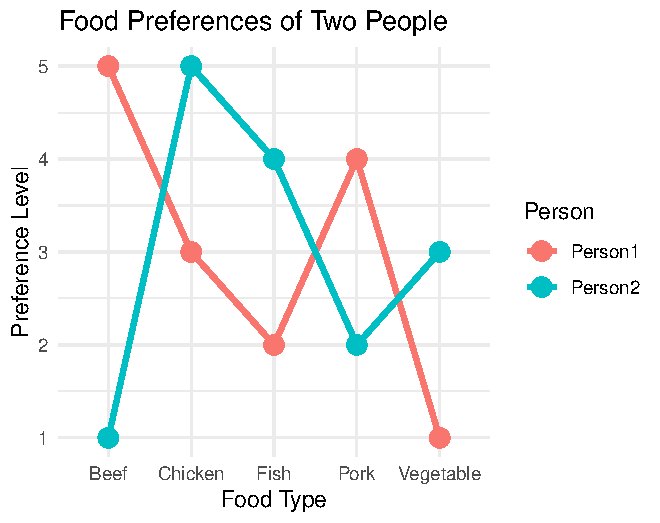
\includegraphics[width=0.6\textwidth]{foodpreference}
	\caption{Food preference for two people}
\end{figure}

The concept of ordinal patterns in time series can be effectively demonstrated through a real-world example. Traditionally, numerous algorithms, techniques, and heuristics have been utilized to estimate complexity measures from real-world data. However, these methods often prove effective only for low-dimensional dynamical systems and struggle to perform well when noise is introduced into the data.

The Bandt and Pompe method overcomes this limitation by offering a robust approach that remains reliable even in noisy environments. In time series analysis, key complexity measures—such as entropy, fractal dimension, and Lyapunov exponents—play a crucial role. These measures are instrumental in comparing neighboring values, helping to uncover the underlying structure and dynamics of the data.

The advantages of Bandt \& Pompe methods:
\begin{itemize}
	\item Simplicity
	\item Extremely fast calculation
	\item Robutness
	\item Invariance with respect to nonlinear monotonous transformation
\end{itemize}	
	
		
One disadvantage of this method is that, although it is extremely fast and robust, it is best suited for large datasets and scenarios where there is limited time for preprocessing or fine-tuning parameters.

However, despite the widespread use of ordinal patterns to study the latent dynamics of time series through permutation entropy, there are no established theoretical results concerning the distribution of permutation entropy that account for the correlation effects between patterns. Nonetheless, Rey et al. \cite{Rey2023a} demonstrated that the asymptotic distribution of permutation entropy is normal. They compared their findings with those of multinomial sample entropy, which assumes independence between patterns. Notably, the expression for the asymptotic variance becomes increasingly complex as the embedding dimension increases. 

This proposal has three objectives in order to continue this research work.
\begin{itemize}
	\item Define a data base of time series for clustering, i.e., finding similar time series. 
	\item Extract all the features we know from their Bandt \& Pompe symbolization (Shannon, Tsallis and Renyi entropies, Fisher information measure, complexities, and the available confidence intervals)
	\item Use those features for time series clustering 
\end{itemize} 




